\documentclass{article}
\usepackage[utf8]{inputenc}
\usepackage[greek,english]{babel}
\usepackage{alphabeta}
\usepackage{fancyhdr}
\usepackage{listings}
\usepackage{mathtools}
\usepackage{siunitx}
\usepackage{xcolor}
\usepackage{graphicx}
\usepackage{pgfplots}
\usepackage[export]{adjustbox}
\usepackage{biblatex}
%\addbibresource{el1-citations.bib}

\title{Εργαστηριακή Ασκηση 1 \& 2} 
\author{Χρήστος Μαργιώλης - 19390133 \\ Τμήμα ΗΛΕΚ03}
\date{Νοέμβριος 2020}

\begin{document}

\begin{figure}[t!]
        \centering
        
\includegraphics[scale=0.3, center]{./res/Logo_University_of_West_Attica.png}
        \Large
        \textbf{Πανεπιστήμιο Δυτικής Αττικής} \\
        \large
        Τμήμα Μηχανικών Πληροφορικής και Ηλεκτρονικών Υπολογιστών \\
        Ηλεκτρονική
\end{figure}
\begin{figure}[b]
        \centering
        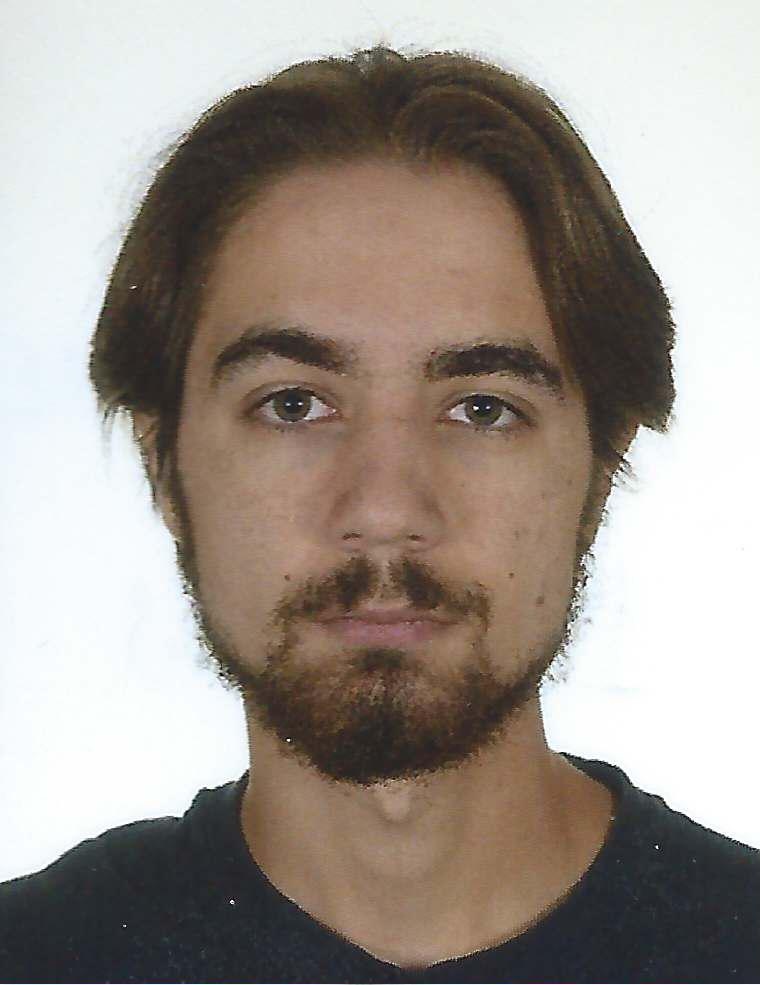
\includegraphics[scale=1]{./res/19390133.jpeg}
\end{figure}

\begin{titlepage}
\maketitle
\end{titlepage}

\renewcommand{\contentsname}{Περιεχόμενα}
\tableofcontents

\renewcommand{\abstractname}{Εισαγωγή}
\begin{abstract}
        Ο σκοπός της εργασίας αυτής είναι η εξοικείωση με μετρήσεις χρησιμοποιώντας
        τον παλμογράφο, καθώς και η κατανόηση της συνεχούς και εναλλασσόμενης τάσης.
\end{abstract}
\pagebreak

\section{Περιγραφή υλοποίησης}
Προκειμένου να υλοποιηθεί η εργασία αυτή χρησιμοποιήθηκε το εργαλείο Multisim για την
συνδεσμολογία κυκλωμάτων καθώς και των μετρήσεων πάνω σε αυτά. Πιο συγκεκριμένα,
το βασικό εργαλείο αυτής της εργασίας είναι ο παλμογράφος και οι A.C και D.C πηγές
τάσης.

\section{Εργαστηριακό μέρος}
\subsection{Μέτρηση συνεχούς τάσης D.C}
Αφού επιλέξουμε μία πηγή 5V D.C τάσης, την συνδέουμε στο παρακάτω
κύκλωμα και συνδέοντας κατάλληλα τον παλμογράφο και το πολύμετρο
βλέπουμε ότι τα αποτελέσματα που προκύπτουν είναι τα παρακάτω.
Παρατηρούμε επίσης ότι και ο παλμογράφος και το πολύμετρο βγάζουν
τα ίδια αποτελέσματα. Τέλος, βλέπουμε ότι ο παλμογράφος εμφανίζει
μία συνεχή γραμμή - αυτό οφείλεται στο ότι η πηγή είναι συνεχούς
τάσης.

\begin{center}
\begin{tabular}{|c|c|}
        \hline
        Eνδειξη παλμογράφου & Eνδειξη βολτόμετρου \\
        \hline
        5V & 5V \\
        \hline
\end{tabular}
\end{center}

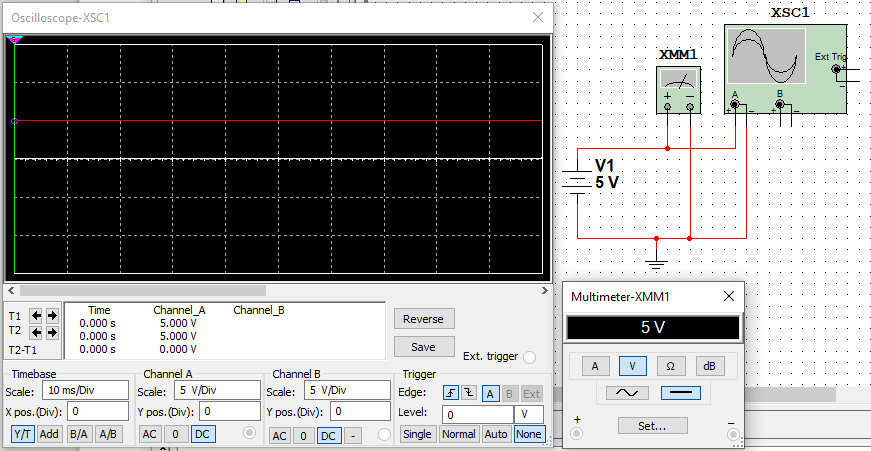
\includegraphics[width=\textwidth]{./res/ex1circ.png} \\

\subsection{Μέτρηση εναλλασσόμενης τάσης A.C}
Αρχικά βάζουμε πηγή εναλλασσόμενης τάσης και την ρυθμίζουμε να
έχει συχνότητα $1000\si{\hertz}$ και έξοδο $1V$. Συνδέοντας το κύκλωμα στον
παλμογράφο παρατηρούμε ότι η τάση στην πάνω κορυφή είναι $1.407V$ και
στην κάτω κορυφή $-1.412V$, οπότε για βρούμε την τάση από κορυφή σε
κορυφή προσθέτουμε τις δύο κορυφές χωρίς να νοιαστούμε για το πρόσιμο
τους. Οπότε
\[V_{p-p} = V_{p1} + V_{p2} = 1.4 + 1.4 = 2.8\]

Εναλλακτικά, θα μπορούσαμε να υπολογίσουμε το $V_{p-p}$ μέσω του
τύπου
%\cite{learnelec}
\[V_{p-p} = V_{rms} \cdot 2\sqrt 2 = 1 \cdot 2\sqrt 2 = 2.8V\]

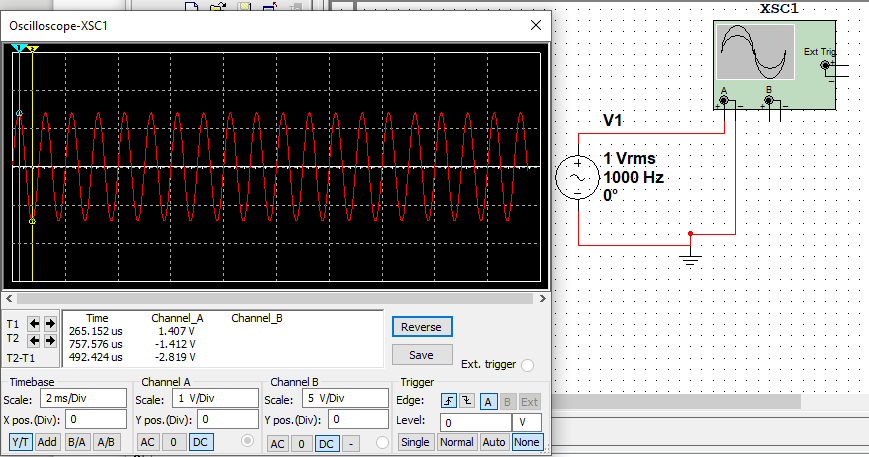
\includegraphics[width=\textwidth]{./res/ex2circ.png} \\

Mε τα παραπάνω δεδομένα και τους τύπους του παρακάτω πίνακα μπορούμε να 
βρούμε και τα υπόλοιπα ζητούμενα:
\[V_p = \frac{V_{p-p}}{2}V = \frac{2.8}{2}V = 1.4V\]
\[V_{εν} = \frac{V_p}{\sqrt 2}V = \frac{1.4}{\sqrt 2}V \approx 0.99V = 1V\]

Συνδέοντας στο κύκλωμα και ένα βολτόμετρο παρατηρούμε ότι η $V_{εν}$ τάση
που προκύπτει είναι πράγματι ίδια με αυτήν που υπολογίσαμε παραπάνω.

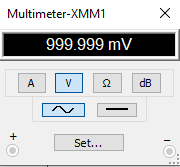
\includegraphics[width=\textwidth / 2,center]{./res/ex2vm.png} \\

Αντίστοιχα, ρυθμίζοντας την έξοδο σε 2 και $2.5V$, καταλήγουμε με
τα παρακάτω αποτελέσματα.

\begin{center}
\begin{tabular}{|p{30mm}|p{30mm}|p{30mm}|p{30mm}|}
        \hline
        Σήμα εισόδου ενεργός τιμή σε Volt &
        Τιμή τάσης $V_{p-p}$ (κορυφή σε κορυφή) σε Volt &
        Υπολογισμός τιμής τάσης $V_p$ σε Volt $V_p = V_{p-p} / 2$ &
        Υπολογισμός ενεργού τιμής $V_{εν}$ σε Volt $V_{εν} = V_p / \sqrt 2$ \\
        \hline
        1 & 2.8 & 1.4 & 1 \\
        \hline
        2 & 5.6 & 2.8 & 2 \\
        \hline
        2.5 & 7.0 & 3.5 & 2.5 \\
        \hline
\end{tabular}
\end{center}

\subsection{Μέτρηση της περιόδου και υπολογισμός της συχνότητας F από αυτήν}
Συνδέουμε γεννήτρια εναλλασσόμενης τάσης και ρυθμίζουμε την συχνότητα σε $1000\si{\hertz}$
και $2.5V_{p}$. Ο λόγος που την ρυθμίζουμε σε $2.5V_{p}$ είναι επειδή 
\[V_p = \frac{V_{p-p}}{2}V \Rightarrow V_p = \frac{5}{2}V \Rightarrow V_p = 2.5V\]
Για να υπολογίσουμε την περίοδο χρησιμοποιούμε τον τύπο 
\[T = \frac{1}{f}\]
Και για την συχνότητα
\[f = \frac{1}{T}\]

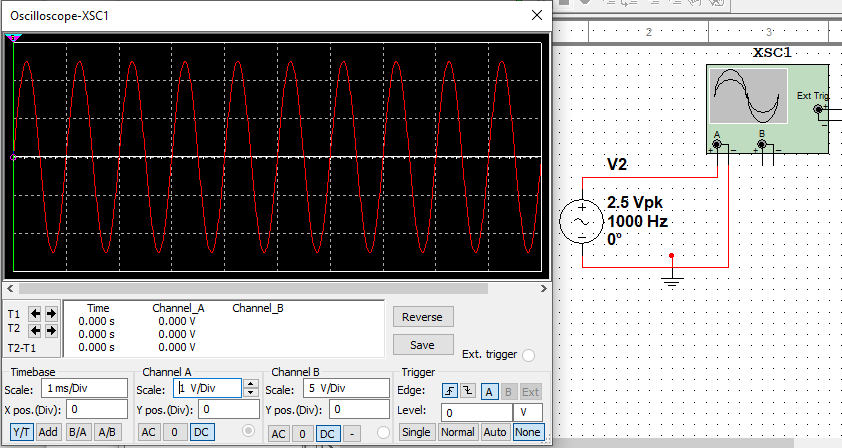
\includegraphics[width=\textwidth]{./res/ex3circ.png} \\

\begin{center}
\begin{tabular}{|c|c|c|}
        \hline
        Συχνότητα  $f / \si{\hertz}$ &
        Περίοδος $T / \si{msec}$ &
        Υπολογισμός συχνότητας \si{\hertz} \\
        \hline
        1000 & $1.016\si{\milli\sec}$ & $10^3 / 1.016 = 984\si{\hertz}$ \\
        \hline
        2000 & $0.5\si{\milli\sec}$ & $10^3 / 0.5 = 2000\si{\hertz}$ \\
        \hline
        3000 & $0.329\si{\milli\sec}$ & $10^3 / 0.329 = 3039\si{\hertz}$ \\
        \hline
        4000 & $0.251\si{\milli\sec}$ & $10^3 / 0.251 = 3984\si{\hertz}$ \\
        \hline
        5000 & $0.203\si{\milli\sec}$ & $10^3 / 0.203 = 4926\si{\hertz}$ \\
        \hline
\end{tabular}
\end{center}

\subsection{Μέτρηση της διαφοράς φάσης}
Όπως και στην παραπάνω άσκηση, θα συνδεσμολογήσουμε το κύκλωμα συνδέοντας
εναλλασσόμενη τάση με έξοδο $V_p = 2.5V$ ($V_{p} = V_{p-p} / 2$) μέγιστη τιμή τάσης. 
Επίσης θα ρυθμίσουμε την συχνότητα σε $500\si{\hertz}$. Για να έχουμε ίσες αποκλίσεις
στους αξόνες πρέπει να ρυθμίσουμε το Scale στο Channel A και Channel B να είναι ίσα,
δηλαδή 1 $Y / DIV$.

Από το παρακάτω κύκλωμα βλέπουμε ότι
\begin{itemize}
        \item
        $α(div) = T2 = 2.39V$
        \item
        $β(div) = T1 = 2.5V$
\end{itemize}
Έχοντας αυτά τα δύο δεδομένα, μπορούμε να υπολογίσουμε την διαφορά φάσης
\[\si{\phi\degree} = \arcsin(α/β) = \arcsin(2.39 / 2.5) = \arcsin(0.956) = 72.94\si{\degree}\]

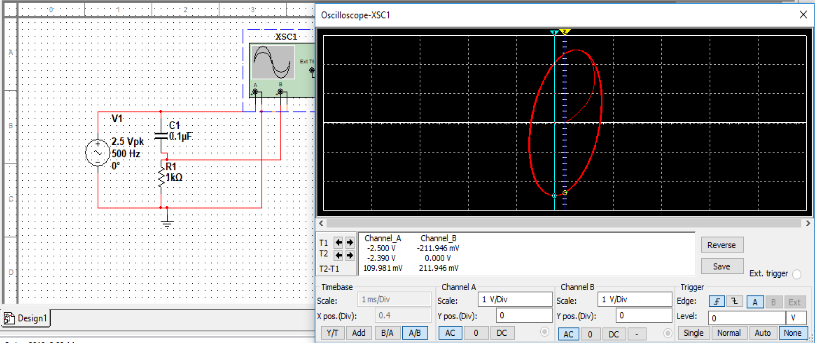
\includegraphics[width=\textwidth]{./res/ex4circ.png} \\

Aλλάζονοτας την ρύθμιση από $A/B$ σε $Y/T$, έχουμε την κυματομορφή
από την οποία μπορούμε να υπολογίσουμε την περίοδο $A(div)$.
\[A(div) = T2 - T1 = 2\si{\milli\sec}\]

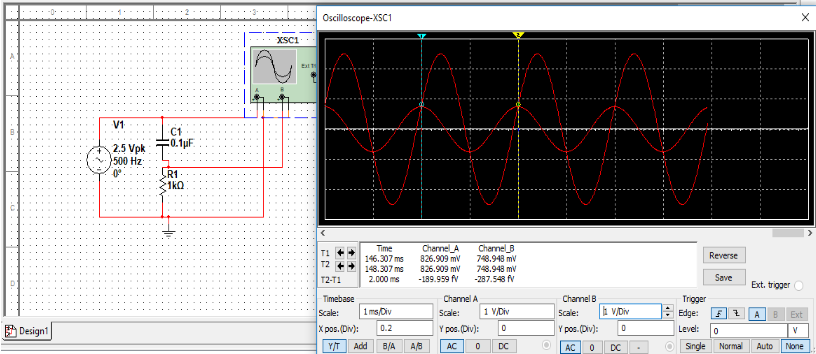
\includegraphics[width=\textwidth]{./res/ex4wave1.png} \\

Για υπολογίσουμε την χρονική διαφορά μεταξύ των δεικτών $B(div)$ θα θέσουμε τους δείκτες
στις κορυφές των δύο κυματομορφών, επομένως
\[B(div) = T2 - T1 = 405.797\si{u\sec} = 0.405\si{\milli\sec}\]

Έχοντας το $B(div)$ μπορούμε επίσης να υπολογίσουμε την διαφορά φάσης με την
απλή μέθοδο των τριών.
\[\si{\phi\degree} = B(div) \cdot \frac{360}{A(div)} = 0.405 \cdot 180 = 72.9\si{\degree}\]

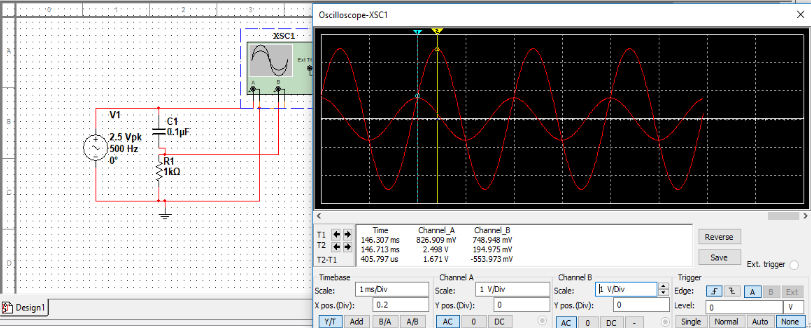
\includegraphics[width=\textwidth]{./res/ex4wave2.png} \\

Για χάρην ευκολίας δεν θα παραθέσω εικόνες από όλες τις μετρήσεις για όλους
του υπόλοιπους συνδυασμούς, διότι η διαδικασία είναι η ίδια, όμως τα αποτελέσματα
των μετρήσεων είναι τα εξής

\begin{center}
        \begin{tabular}{|c|p{10mm}|p{10mm}|p{30mm}|c|c|p{30mm}|}
        \hline
        Συχνότητα \si{\hertz} &
        $A (div) \newline (\si{\milli\sec)}$ &
        $B (div) \newline (\si{\milli\sec})$ &
        Διαφορά φάσης \newline (απλή μέθοδος των τριών) \si{\phi\degree} &
        $α (div) (V)$ & $β (div) (V)$ &
        Διαφορά φάσης \newline ($\arcsin(α/β)$) \si{\phi\degree} \\
        \hline
        500 & 2 & 0.405 & 72.9 & 2.39 & 2.5 & 72.94 \\
        \hline
        1000 & 1 & 0.1621 & 58.35 & 2.131 & 2.5 & 58.42 \\
        \hline
        2000 & 0.5 & 0.005 & 36 & 1.463 & 2.5 & 35.8 \\
        \hline
        3000 & 0.333 & 0.0261 & 28.2 & 1.164 & 2.5 & 27.75 \\
        \hline
        4000 & 0.25 & 0.015 & 21.6 & 0.913 & 2.5 & 21.4 \\
        \hline
        5000 & 0.2 & 0.00942 & 16.95 & 0.745 & 2.5 & 17.3 \\
        \hline
\end{tabular}
\end{center}

\subsection{Ερωτήσεις}
\subsubsection{Ερώτηση 1}
Ποιά η τιμή της συνεχούς τάσης που προκαλεί απόκλιση του στίγματος
3 τετραγωνάκια και ο μεταγωγέας $Volt / DIV$ είναι στη θέση 2; \\

\textit{Απάντηση}: Εφόσον ο μεταγωγέας είναι στην θέση 2, τότε κάθε
τετραγωνάκι αναπαριστά $2V$, οπότε η τιμή τάσης είναι
$2V \cdot$ απόκλιση στίγματος $\Rightarrow 2V \cdot 3 = 6V$

\subsubsection{Ερώτηση 2}
Ποιές οι τιμές της εναλλασσόμενης τάσης $V_{p-p}$, $V_p$ και $V_{εν}$,
η οποία προκαλεί απόκλιση του στίγματος 0.5, 2 και 3 τετραγωνάκια αντίστοιχα
από κορυφή σε κορυφή και ο μεταγωγέας $Volt / DIV$ είναι στη θέση $50mV$,
$2V$ και $5V$ αντίστοιχα; \\

\textit{Απάντηση}: Ακολουθώντας την λογική της ερώτησης 1 μπορούμε
να συμπεράνουμε ότι: \\
$V_{p-p} =$ μεταγωγέας $\cdot$ απόκλιση$_{p-p}$ \\
Επίσης γνωρίζουμε ότι: \\
$V_p = V_{p-p} / 2$ \\
$V_{εν} = V_p / \sqrt 2$ \\
Χρησιμοποιώντας τους παραπάνω τύπους και αντικαθιστώντας με τα δεδομένα
της εκφώνησης, μπορούμε να καταγράψουμε τα αποτελέσματα στον παρακάτω
πίνακα

\begin{center}
\begin{tabular}{|p{20mm}|c|c|c|c|c|c|c|c|c|}
        \hline
        &
        \multicolumn{3}{p{27mm}|}{Απόκλιση$_{p-p}$ 0.5 τετραγωνάκια} &
        \multicolumn{3}{p{27mm}|}{Απόκλιση$_{p-p}$ 2 τετραγωνάκια} &
        \multicolumn{3}{p{27mm}|}{Απόκλιση$_{p-p}$ 3 τετραγωνάκια} \\
        \hline
        Μεταγωγέας $Volt / Div$ & $V_{p-p}$ & $V_p$ & $V_{εν}$ &
        $V_{p-p}$ & $V_p$ & $V_{εν}$ &
        $V_{p-p}$ & $V_p$ & $V_{εν}$ \\
        \hline
        $50mV$ & 0.025 & 0.0125 & 0.009 & 0.1 & 0.05 & 0.035 & 0.15 & 0.075 & 0.053 \\
        \hline
        $2V$ & 1 & 0.5 & 0.353 & 4 & 2 & 1.414 & 6 & 3 & 2.121 \\
        \hline
        $5V$ & 2.5 & 1.25 & 0.884 & 10 & 5 & 3.535 & 15 & 7.5 & 5.302 \\
        \hline
\end{tabular}
\end{center}

\subsubsection{Ερώτηση 3}
Ποιά η συχνότητα της εναλλασσόμενης τάσης όταν η απόκλιση από κορυφή
σε κορυφή είναι 0.5, 2 και 3 τετραγωνάκια και ο μεταγωγέας $Time / DIV$ είναι στη
θέση 2, 5 και $50ms$ αντίστοιχα; \\

\textit{Απάντηση}: Πάλι ακολουθώντας παρόμοια λογική με τις δύο παραπάνω ερωτήσεις,
μπορούμε να χρησιμοποιήσουμε τα δεδομένα της εκφώνησης ώστε να βρούμε τον τύπο της
περιόδου και της συχνότητας και στην συνέχεια να καταγράψουμε τα αποτελέσματα 
στον παρακάτω πίνακα. Η περίοδος είναι: \\
$T =$ μεταγωγέας $\cdot$ απόκλιση$_{p-p}$ \\
Επίσης γνωρίζουμε ότι ο τύπος της συχνότητας είναι: \\
$f = 1 / T$ \\
Έτσι μπορούμε να υπολογίσουμε τα αποτελέσματα με βάση τα παραπάνω δεδομένα.

\begin{center}
\begin{tabular}{|p{20mm}|c|c|c|c|c|c|}
        \hline
        &
        \multicolumn{2}{p{27mm}|}{Απόκλιση$_{p-p}$ 0.5 τετραγωνάκια} &
        \multicolumn{2}{p{27mm}|}{Απόκλιση$_{p-p}$ 2 τετραγωνάκια} &
        \multicolumn{2}{p{27mm}|}{Απόκλιση$_{p-p}$ 3 τετραγωνάκια} \\
        \hline
        Μεταγωγέας $Volt / Div$ & $T(ms)$ & $f(\si{\hertz})$ &
        $T(ms)$ & $f(\si{\hertz})$ & $T(ms)$ & $f(\si{\hertz})$ \\
        \hline
        $2 ms$ & 1 & 1000 & 4 & 250 & 6 & 167 \\
        \hline
        $5 ms$ & 2.5 & 400 & 10 & 100 & 15 & 67 \\
        \hline
        $50 ms$ & 25 & 40 & 100 & 10 & 150 & 7 \\
        \hline
\end{tabular}
\end{center}

\subsubsection{Ερώτηση 4}
Ποιά η διαφορά φάσης δύο εναλλασσόμενων κυματομορφών τάσεων όταν απέχουν
χρονικά μεταξύ τους 1.5 τετραγωνάκια και η απόσταση μεταξύ δύο συνεχόμενων
κορυφών της μίας κυματομορφής είναι 6 τετραγωνάκια; \\

\textit{Απάντηση}: Χρησιμοποιώντας της απλή μέθοδο των τριών έχουμε ότι: \\
6 τετραγωνάκια = $360\si{\degree}$ \\
1.5 τετραγωνάκια = $x\si{\degree}$ \\
Οπότε
\[x = 360 \si{\degree} \cdot \frac{1.5}{6} \Rightarrow x = 360\si{\degree} \cdot 0.25
        \Rightarrow x = 90\si{\degree}\]

\subsubsection{Ερώτηση 5}
Να υπολογίσετε θεωρητικά αναμενόμενες τιμές της διαφοράς φάσης $\phi$
χρησιμοποιώντας τον τύπο $\phi = \arctan(1 / (2 \pi f RC))$ και τις 6 τιμές
της συχνότητας από τον πίνακα 3 γνωρίζοντας ότι: \\
$\pi = 3.14$ \\
$f$ η συχνότητα της εναλλασσόμενης τάσης για την οποία έγινε η μέτρηση \\
$R = 1\si{\kohm}$ η αντίσταση που χρησιμοποιήθηκε για την κατασκευή του κυκλώματος \\
$C = 0.1\si{\mu\farad}$ η χωρητικότητα που χρησιμοποιήθηκε για την κατασκευή του κυκλώματος \\
Κατόπιν να συγκρίνετε τις θεωρητικές τιμές με αυτές του πίνακα 3. \\

\textit{Απάντηση}: Αρχικά πρέπει να υπολογίσουμε την τιμή του $2\pi RC$:

\[2\pi RC = 2 \cdot 3.14 \cdot 1\si{\kohm} \cdot 0.1\si{\mu\farad} =
        6.28 \cdot 1000 \cdot 0.0000001 = 0.000628\]

Έπειτα θα πάρουμε τις συχνότητες από τον πίνακα της άσκησης 4 ώστε να υπολογίσουμε το $\phi$
αντικαθιστώντας το $f$ στον τύπο $2\pi fRC$ με την εκάστοτε συχνότητα.

\[f = 500\si{\hertz}: \phi = \arctan(1 / (2\pi fRC)) = \arctan(1 / (0.000628 \cdot 500)) =
        \arctan(1 / 0.314) = 72.5\si{\degree}\]
\[f = 1000\si{\hertz}: \phi = \arctan(1 / (2\pi fRC)) = \arctan(1 / (0.000628 \cdot 1000)) =
        \arctan(1 / 0.628) = 57.9\si{\degree}\]
\[f = 2000\si{\hertz}: \phi = \arctan(1 / (2\pi fRC)) = \arctan(1 / (0.000628 \cdot 2000)) =
        \arctan(1 / 1.256) = 38.5\si{\degree}\]
\[f = 3000\si{\hertz}: \phi = \arctan(1 / (2\pi fRC)) = \arctan(1 / (0.000628 \cdot 3000)) =
        \arctan(1 / 1.884) = 27.95\si{\degree}\]
\[f = 4000\si{\hertz}: \phi = \arctan(1 / (2\pi fRC)) = \arctan(1 / (0.000628 \cdot 4000)) =
        \arctan(1 / 2.512) = 21.7\si{\degree}\]
\[f = 5000\si{\hertz}: \phi = \arctan(1 / (2\pi fRC)) = \arctan(1 / (0.000628 \cdot 5000)) =
        \arctan(1 / 3.14) = 17.66\si{\degree}\]

Στην συνέχεια τοποθετούμε όλα τα παραπάνω αποτέλεσματα στον παρακάτω πίνακα

\begin{center}
\begin{tabular}{|c|p{30mm}|p{25mm}|c|}
        \hline
        Συχνοτητα $\si{\hertz}$ &
        Διαφορά φάσης (απλή μέθοδος των τριών) ($\si{\phi\degree}))$ &
        Διαφορά φάσης ($\arcsin(α/β)$) ($\si{\phi\degree}$) &
        $\phi = \arctan(1 / (2\pi fRC))$ \\
        \hline
        500 & 72.9 & 72.94 & 72.5\si{\degree} \\
        \hline
        1000 & 58.35 & 58.42 & 57.9\si{\degree} \\
        \hline
        2000 & 36 & 35.8 & 38.5\si{\degree} \\
        \hline
        3000 & 28.2 & 27.75 & 27.95\si{\degree} \\
        \hline
        4000 & 21.6 & 21.4 & 21.7\si{\degree} \\
        \hline
        5000 & 16.95 & 17.3 & 17.66\si{\degree} \\
        \hline
\end{tabular}
\end{center}

\renewcommand\refname{Πηγές}
%\printbibliography
\end{document}
